\chapter*{Dodatak: Prikaz aktivnosti grupe}
		\addcontentsline{toc}{chapter}{Dodatak: Prikaz aktivnosti grupe}
		
		\section*{Dnevnik sastajanja}
		
		\newcommand{\imenaSvihClanova}{M. Benotić, P. Jakopec, M. Lazarić, A. Novak, R. Pavliš, I. Teofilović, F. Vale}
		
		\begin{packed_enum}
			\item  sastanak
			\item[] \begin{packed_item}
				\item Datum: 9. listopada 2019.
				\item Prisustvovali: \imenaSvihClanova
				\item Teme sastanka:
				\begin{packed_item}
					\item upoznavanje članova
					\item definiranje rokova
				\end{packed_item}
			\end{packed_item}
		
			\item  sastanak
			\item[] \begin{packed_item}
				\item Datum: 15. listopada 2019.
				\item Prisustvovali: \imenaSvihClanova
				\item Teme sastanka:
				\begin{packed_item}
					\item određivanje funkcionalnih i nefunkcionalnih zahtjeva aplikacije
					\item prioritizacija zahtjeva
				\end{packed_item}
			\end{packed_item}
		
			\item  sastanak
			\item[] \begin{packed_item}
				\item Datum: 17. listopada 2019.
				\item Prisustvovali: \imenaSvihClanova
				\item Teme sastanka:
				\begin{packed_item}
					\item određivanje funkcionalnih i nefunkcionalnih zahtjeva aplikacije
					\item prioritizacija zahtjeva
					\item odabir tehnologije za izradu web aplikacije
				\end{packed_item}
			\end{packed_item}
		
			\item  sastanak
			\item[] \begin{packed_item}
				\item Datum: 22. listopada 2019.
				\item Prisustvovali: \imenaSvihClanova
				\item Teme sastanka:
				\begin{packed_item}
					\item razrada specifikacije programske potpore
					\item obrasci uporabe i sekvencijski dijagrami
				\end{packed_item}
			\end{packed_item}
		
			\item  sastanak
			\item[] \begin{packed_item}
				\item Datum: 29. listopada 2019.
				\item Prisustvovali: \imenaSvihClanova
				\item Teme sastanka:
				\begin{packed_item}
					\item baza podataka
					\item komentiranje dosadašnje verzije dokumentacije
				\end{packed_item}
			\end{packed_item}
		
			\item  sastanak
			\item[] \begin{packed_item}
				\item Datum: 5. studenog 2019.
				\item Prisustvovali: M. Lazarić, R. Pavliš, F. Vale
				\item Teme sastanka:
				\begin{packed_item}
					\item komentiranje obrazaca uporabe i sekvencijskih dijagrama
				\end{packed_item}
			\end{packed_item}
		
			\item  sastanak
			\item[] \begin{packed_item}
				\item Datum: 12. studenog 2019.
				\item Prisustvovali: \imenaSvihClanova
				\item Teme sastanka:
				\begin{packed_item}
					\item komentiranje dosadašnje verzije dokumentacije
					\item demonstracija generičkih funkcionalnosti
				\end{packed_item}
			\end{packed_item}
			
			\item  sastanak
			\item[] \begin{packed_item}
				\item Datum: 10. prosinca 2019.
				\item Prisustvovali: \imenaSvihClanova
				\item Teme sastanka:
				\begin{packed_item}
					\item podjela poslova na dokumentaciji i samoj aplikaciji
					\item rasprava o preostalim poglavljima dokumentacije
				\end{packed_item}
			\end{packed_item}
			
			\item  sastanak
			\item[] \begin{packed_item}
				\item Datum: 17. prosinca 2019.
				\item Prisustvovali: \imenaSvihClanova
				\item Teme sastanka:
				\begin{packed_item}
					\item rad sa Selenium testovima
				\end{packed_item}
			\end{packed_item}
			
			\item  sastanak
			\item[] \begin{packed_item}
				\item Datum: 7. siječnja 2020.
				\item Prisustvovali: \imenaSvihClanova
				\item Teme sastanka:
				\begin{packed_item}
					\item demonstracija alfa inačice aplikacije
				\end{packed_item}
			\end{packed_item}
			
			\item  sastanak
			\item[] \begin{packed_item}
				\item Datum: 14. siječnja 2020.
				\item Prisustvovali: \imenaSvihClanova
				\item Teme sastanka:
				\begin{packed_item}
					\item završno komentiranje dokumentacije
					\item konačna dorada dokumentacije
				\end{packed_item}
			\end{packed_item}
			
		\end{packed_enum}
		
		\eject
		\section*{Tablica aktivnosti}

			\begin{longtabu} to \textwidth {|X[7, l]|X[1, c]|X[1, c]|X[1, c]|X[1, c]|X[1, c]|X[1, c]|X[1, c]|}
								
				\cline{2-8} \multicolumn{1}{c|}{\textbf{}} &     \multicolumn{1}{c|}{\rotatebox{90}{\textbf{Marko Lazarić }}} & \multicolumn{1}{c|}{\rotatebox{90}{\textbf{Aleksandar Novak }}} &	\multicolumn{1}{c|}{\rotatebox{90}{\textbf{Filip Vale }}} &	\multicolumn{1}{c|}{\rotatebox{90}{\textbf{Ivan Teofilović }}} &
				\multicolumn{1}{c|}{\rotatebox{90}{\textbf{Matija Benotić }}} &
				\multicolumn{1}{c|}{\rotatebox{90}{\textbf{Petar Jakopec }}} &	\multicolumn{1}{c|}{\rotatebox{90}{\textbf{Robert Pavliš }}} \\ \hline 
				\endfirsthead
				
			
				\cline{2-8} \multicolumn{1}{c|}{\textbf{}} &     \multicolumn{1}{c|}{\rotatebox{90}{\textbf{Marko Lazarić }}} & \multicolumn{1}{c|}{\rotatebox{90}{\textbf{Aleksandar Novak }}} &	\multicolumn{1}{c|}{\rotatebox{90}{\textbf{Filip Vale }}} &
				\multicolumn{1}{c|}{\rotatebox{90}{\textbf{Ivan Teofilović }}} &	\multicolumn{1}{c|}{\rotatebox{90}{\textbf{Matija Benotić }}} &
				\multicolumn{1}{c|}{\rotatebox{90}{\textbf{Petar Jakopec }}} &	\multicolumn{1}{c|}{\rotatebox{90}{\textbf{Robert Pavliš }}} \\ \hline 
				\endhead
				
				
				\endfoot
							
				 
				\endlastfoot
				
				Upravljanje projektom 		& 11 & 9 & 10 & 9 & 9 & 10 & 10 \\ \hline
				Opis projektnog zadatka 	& 2 & 1 & 1 & -  & - & 2 & 2 \\ \hline
				
				Funkcionalni zahtjevi       & - & - & - & - & 2 & - & -  \\ \hline
				Opis pojedinih obrazaca 	& - & 1 & 2 & - & - & 2 & 2 \\ \hline
				Dijagram obrazaca 			& - & - & 2 & 2 & - & - & - \\ \hline
				Sekvencijski dijagrami 		& - & - & 1 & - & 2 & 2 & 2 \\ \hline
				Opis ostalih zahtjeva 		& 1 & - & - & 1 & - & - & - \\ \hline

				Arhitektura i dizajn sustava & - & - & - & - & - & 3 & -  \\ \hline
				Baza podataka				& 2 & - & 3 & - & - & - & -  \\ \hline
				Dijagram razreda 			& 3 & - & - & - & - & 1 & -  \\ \hline
				Dijagram stanja				& - & - & 3 & - & - & - & - \\ \hline
				Dijagram aktivnosti 		& - & - & 3 & - & - & - & -\\ \hline
				Dijagram komponenti			& - & - & - & - & 4 & - & - \\ \hline
				Korištene tehnologije i alati 		& - & - & - & - & - & - & 4 \\ \hline
				Ispitivanje programskog rješenja 	& 6 & - & - & - & 5 & - & - \\ \hline
				Dijagram razmještaja			& - & - & - & 3 & - & - & -  \\ \hline
				Upute za puštanje u pogon 		& - & - & - & - & - & 4 & - \\ \hline 
				Dnevnik sastajanja 			& 1 & - & 4 & - & - & - & - \\ \hline
				Zaključak i budući rad 		& - & - & - & - & - & - & 3 \\  \hline
				Popis literature 			& - & - & - & - & - & - & - \\  \hline
				Autentikacija 			& - & 3 & - & - & 3 & - & - \\ \hline
				Frontend 				& - & 10 & - & - & - & - & - \\  \hline
				Backend 				& 5 & - & - & - & - & - & - \\  \hline
			\end{longtabu}
					
					
		\eject
		\section*{Dijagrami pregleda promjena}

		\begin{figure}[H]
    					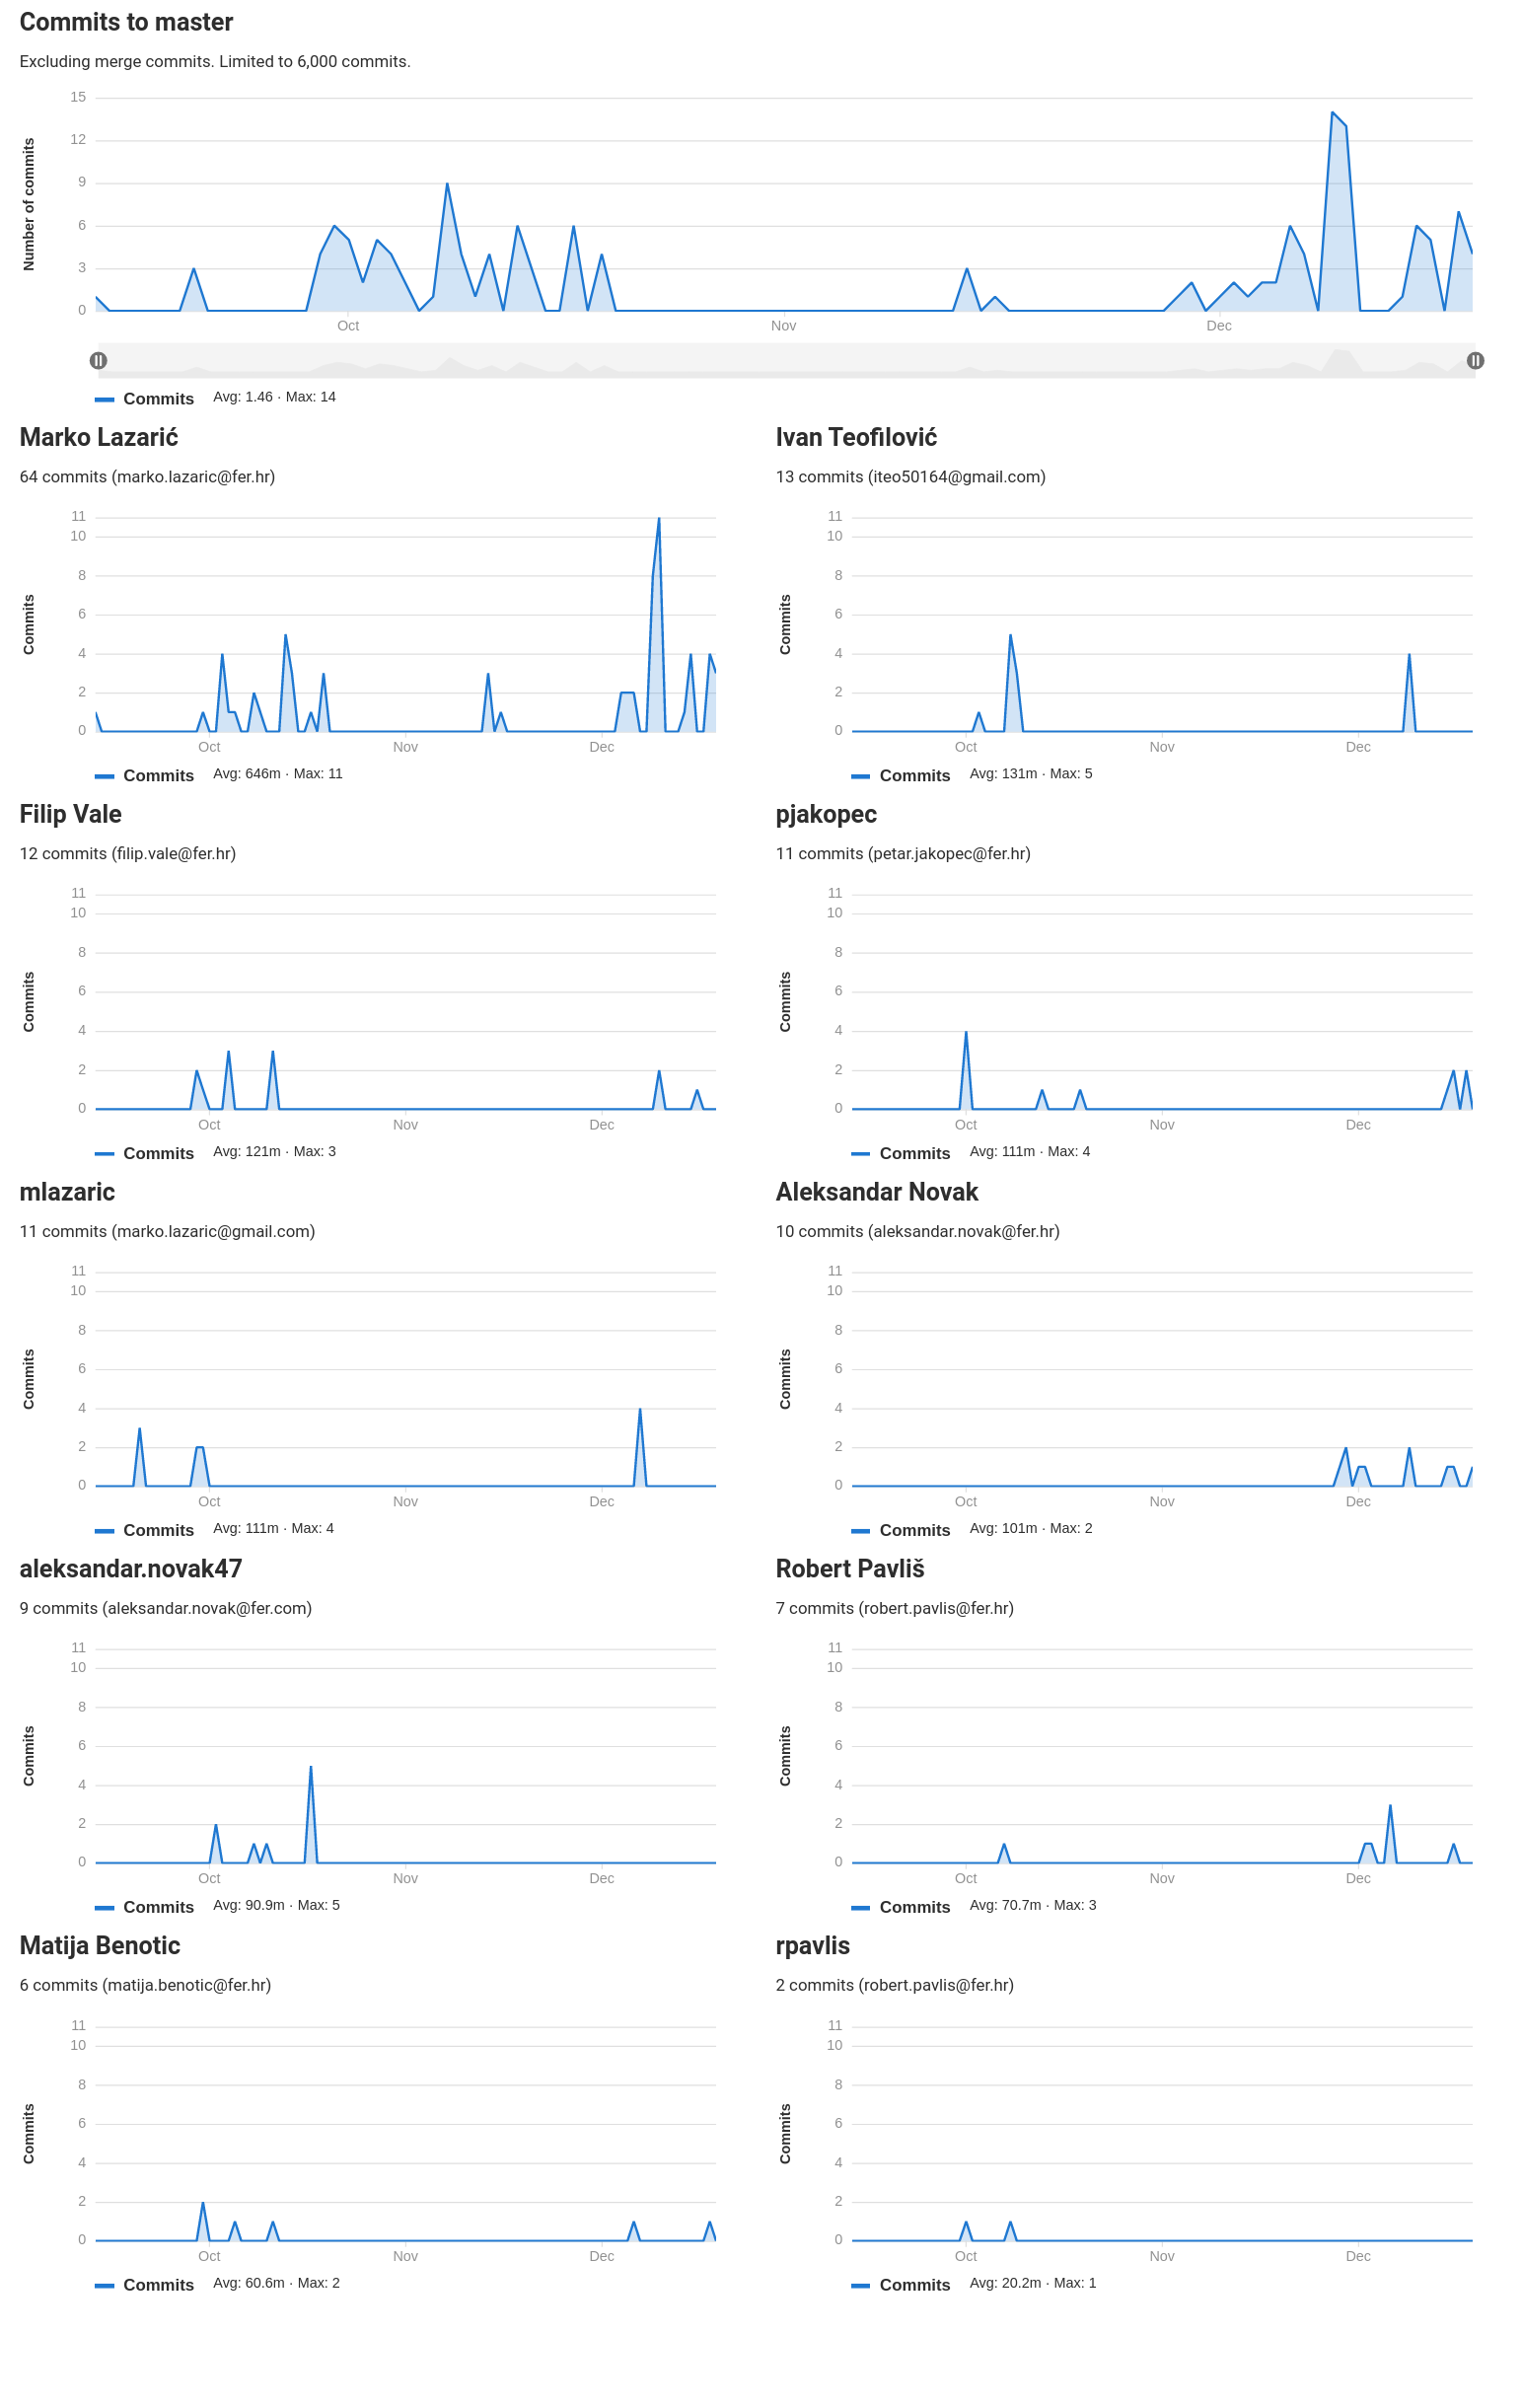
\includegraphics[width=\textwidth,height=0.9\textheight,keepaspectratio]{slike/aktivnost}
    					\centering
    					\caption{Prikaz aktivnosti na repozitoriju}
    					\label{fig:aktivnost}
    		            \end{figure}
		
		
		% \textbf{\textit{dio 2. revizije}}\\
		
		% \textit{Prenijeti dijagram pregleda promjena nad datotekama projekta. Potrebno je na kraju projekta generirane grafove s gitlaba prenijeti u ovo poglavlje dokumentacije. Dijagrami za vlastiti projekt se mogu preuzeti s gitlab.com stranice, u izborniku Repository, pritiskom na stavku Contributors.}
		
	